\section{Overview}
\label{sec:appendix_section}
Supplementary material goes here.
This supplementary material presents additional results to complement the main manuscript. In Section \ref{sec:Implementation}, we detail our coarse-to-fine training strategy, along with the network architectures of the deformable Gaussian MLP and deformable reflection MLP. Subsequently, Section \ref{sec:result} presents additional results, including comprehensive comparisons, more visualizations, and training and rendering efficiency. Finally, in Section \ref{sec:limit}, we discuss the limitation of our approach and provide visual example of failure case. 



\section{Implementation Details}~\label{sec:Implementation} We use PyTorch as our framework and 3DGS~\citep{kerbl20233d} as our codebase. Our coarse-to-fine training strategy is divided into three sequential stages: static, dynamic, and specular stages. 
\paragraph{Static stage.} 
In the static stage, we train the vanilla 3D Gaussian Splatting (3DGS) for 3000 iterations to stabilize the static geometry. 
\paragraph{Dynamic stage.} 
After the static stage, we move on to the dynamic stage. During this phase, we introduce a deformable Gaussian MLP to model dynamic objects. First, we optimize both the canonical Gaussians and the deformable Gaussian MLP for 3,000 iterations until the scene reaches a relatively stable state. Then, we introduce the normal loss $\mathcal{L}_{\text{normal}}$, enabling simultaneous optimization of the scene's normal and depth, and perform an additional 3,000 iterations to further refine the geometry.  The dynamic stage comprises a total of 6,000 training iterations.
\paragraph{Specular stage.} 
After the dynamic stage concludes, we transition to the specular stage, which involves changing the color representation from complete spherical harmonics to $\mathbf{c}_\mathbf{final}$. To mitigate potential geometry disruptions due to the initially incomplete $\mathbf{c}_\mathbf{final}$, we fix the deformable Gaussian MLP and all 3D Gaussian attributes except for zero-order SH, specular tint, and roughness, while temporarily suspending densification. After 6000 iterations, once $\mathbf{c}_\mathbf{final}$ becomes more complete, we resume optimization of all parameters and reinstate the densification process. Then, after another 3000 iterations, we stop the densification process. Concurrently, during the first 2000 iterations of the specular stage, we optimize only the canonical environment map to learn time-invariant lighting. For the canonical environment map, we use $6 \times 128 \times 128$ learnable parameters. Subsequently, we begin optimizing the deformable reflection MLP to capture time-varying lighting effects until the training is complete. The specular stage comprises a total of 31,000 training iterations. For the Peel Banana scene in the HyperNeRF dataset, we do not fix the deformable Gaussian MLP. We resume optimization of all parameters and reinstate the densification process after the first 4000 iterations of the specular stage. Then, after another 2000 iterations, we stop the densification process to prevent excessive growth in the number of 3D Gaussians, which could lead to GPU out-of-memory issues.

For the entire experiment, we train for a total of 40,000 iterations and we use Adam optimizer.


\subsection{Network Architecture of the Deformable Gaussian MLP and Deformable reflection MLP}
\begin{figure}[t]
    \centering
    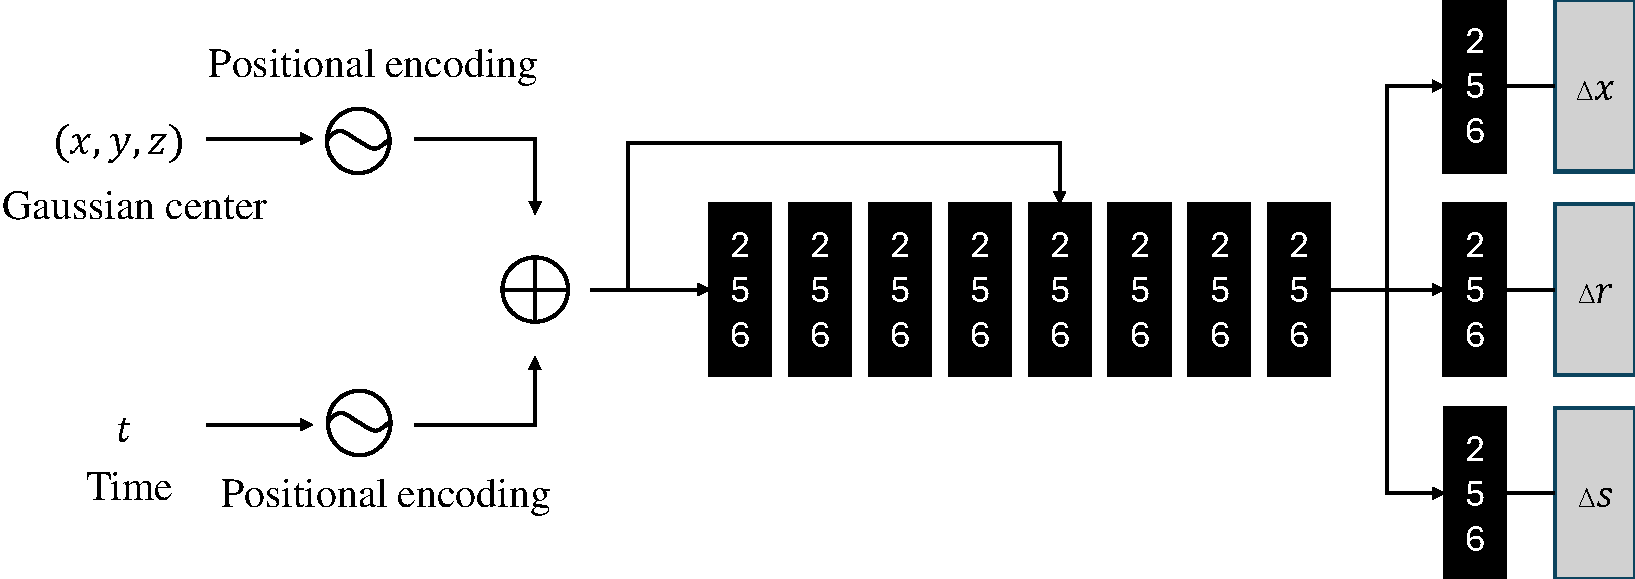
\includegraphics[width=1\linewidth]{figures/deformation_field.pdf}
    \caption{\textbf{ Architecture of the deformable Gaussian MLP}}
    \label{fig:deform_network}
\end{figure}
\begin{figure}[t]
    \centering
    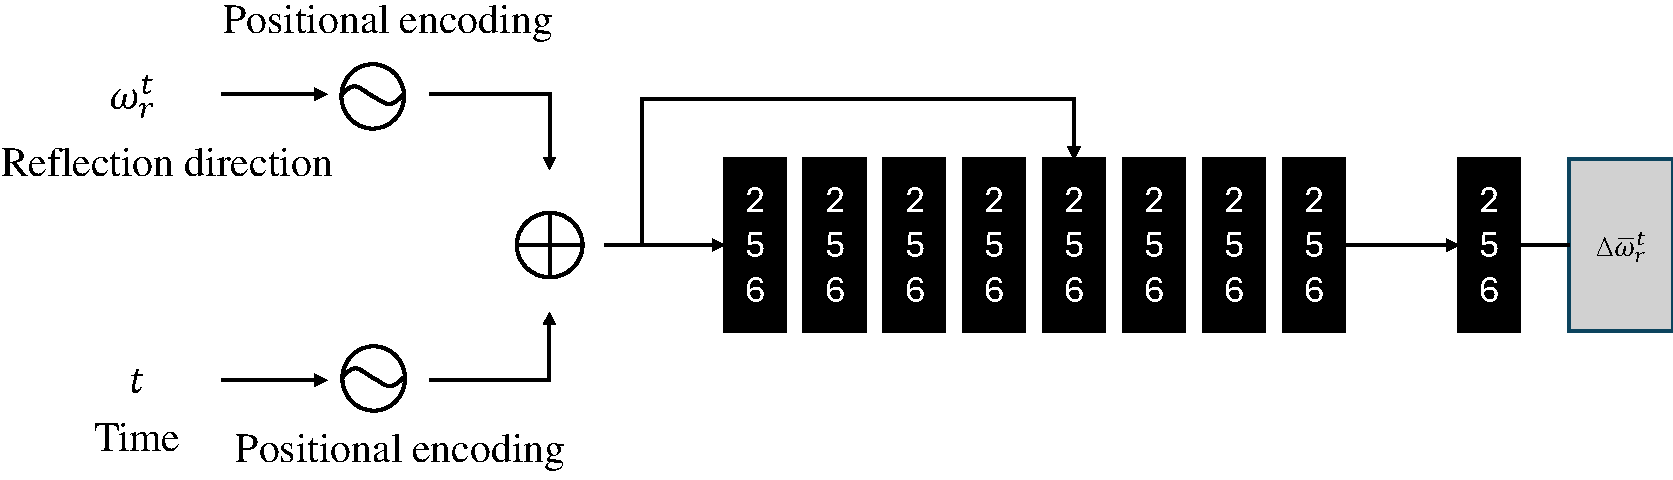
\includegraphics[width=1\linewidth]
    {figures/deformable_reflection.pdf}
    \caption{\textbf{ Architecture of the deformable reflection MLP}}
    \label{fig:deform_refl}
\end{figure}
We follow Deformable 3DGS~\citep{yang2023deformable} and use deformable Gaussian MLP to predict each coordinate of 3D Gaussians and time to their corresponding deviations in position, rotation, and scaling. As shown in Fig. ~\ref{fig:deform_network}, the MLP initially processes the input through eight fully connected layers that employ ReLU activations, featuring 256-dimensional hidden layers and outputs a 256-dimensional feature vector. This vector is then passed through three additional fully connected layers combined with ReLU activation to separately output the offsets over time for position, rotation, and scaling. Notably, similar to NeRF, the feature vector and the input are concatenated in the fourth layer. For the deformable reflection MLP, we utilize the same network architecture, as shown in Fig.~\ref{fig:deform_refl}.

\section{Additional Results}~\label{sec:result}
\subsection{Dynamic specular object of NeRF-DS dataset.}
\begin{table*}[t]
    \setlength{\tabcolsep}{3pt}
    \centering
    % \tiny
    \caption{\textbf{Quantitative comparison on the NeRF-DS~\citep{yan2023nerf} dataset with our labeled dynamic specular masks.} We report PSNR, SSIM, and LPIPS (VGG) of previous methods on dynamic specular objects using the dynamic specular objects mask generated by Track Anything~\citep{yang2023track}. The \colorbox{red!25}{best}, the \colorbox{orange!25}{second best}, and \colorbox{yellow!25}{third best} results are denoted by red, orange, yellow. }
    \label{tab:dynamic_spec_tab}
    \resizebox{\textwidth}{!}{%
    \begin{tabular}{lccccccccccccccc}
    \toprule
     & \multicolumn{3}{c}{As} & &\multicolumn{3}{c}{Basin}& &\multicolumn{3}{c}{Bell}& &\multicolumn{3}{c}{Cup} \\ \cmidrule{2-4} \cmidrule{6-8} \cmidrule{10-12} \cmidrule{14-16}
    Method & PSNR↑ & SSIM↑& LPIPS↓& &PSNR↑ & SSIM↑& LPIPS↓& &PSNR↑ & SSIM↑& LPIPS↓& &PSNR↑ & SSIM↑& LPIPS↓  \\ 
    \midrule
    Deformable 3DGS~\citep{yang2023deformable} &\colorbox{orange!25}{24.14}  &\colorbox{yellow!25}{0.7432 } &\colorbox{orange!25}{0.2957} & &17.45  &0.5530  &\colorbox{orange!25}{0.3138} & &\colorbox{orange!25}{19.42}  &\colorbox{orange!25}{0.5516} &\colorbox{orange!25}{0.2940} & &\colorbox{orange!25}{20.10}  &\colorbox{red!25}{0.5446} &\colorbox{red!25}{0.3312}   \\ 
    4DGS~\citep{wu20234d} &22.70  &0.6993  &\colorbox{yellow!25}{0.3517 }& &16.61 &0.4797  &\colorbox{yellow!25}{0.4084} & &14.64  &\colorbox{yellow!25}{0.2596} &\colorbox{yellow!25}{0.4467 }& &18.90  &0.4132 &0.4032   \\
    GaussianShader~\citep{jiang2023gaussianshader} &19.27  &0.5652  &0.5232 & &15.71 &0.4163  &0.5941 & &12.10  &0.1676 &0.6764 & &14.90  &0.3634 &0.6146   \\
    GS-IR~\citep{liang2023gs} &19.32  &0.5857  &0.4782 & &15.21 &0.4009  &0.5644 & &12.09  &0.1757 &0.6722 & &14.80  &0.3445 &0.6046   \\
    NeRF-DS~\citep{yan2023nerf}&\colorbox{yellow!25}{23.67 }&\colorbox{orange!25}{0.7478}  &0.3635 & &\colorbox{orange!25}{17.98} &\colorbox{yellow!25}{0.5537} &0.4211  & &\colorbox{yellow!25}{14.73} &0.2439 &0.5931  & &\colorbox{yellow!25}{19.95} &\colorbox{yellow!25}{0.5079 }&\colorbox{yellow!25}{0.3494}\\
    HyperNeRF~\citep{park2021hypernerf}&17.37  &0.6934  &0.3834 & &\colorbox{red!25}{18.75} &\colorbox{orange!25}{0.5671}  &0.4125 & &13.93  &0.2292 &0.6051 & &15.07  &0.4860 &0.4183   \\
    Ours &\colorbox{red!25}{24.51} &\colorbox{red!25}{0.7534}  &\colorbox{red!25}{0.2896}  & &\colorbox{yellow!25}{17.71 }&\colorbox{red!25}{0.5675} & \colorbox{red!25}{0.3048}&  &\colorbox{red!25}{19.60} &\colorbox{red!25}{0.5680} &\colorbox{red!25}{0.2862}  & &\colorbox{red!25}{20.13} &\colorbox{orange!25}{0.5384} & \colorbox{orange!25}{0.3368}    \\ 
    \midrule
     & \multicolumn{3}{c}{Plate} & &\multicolumn{3}{c}{Press}& &\multicolumn{3}{c}{Sieve}& &\multicolumn{3}{c}{\textbf{Mean}} \\ \cmidrule{2-4} \cmidrule{6-8} \cmidrule{10-12} \cmidrule{14-16}
    Method & PSNR↑ & SSIM↑& LPIPS↓& &PSNR↑ & SSIM↑& LPIPS↓& &PSNR↑ & SSIM↑& LPIPS↓& &PSNR↑ & SSIM↑& LPIPS↓  \\ 
    \midrule
    Deformable 3DGS~\citep{yang2023deformable} &\colorbox{orange!25}{16.12}  &\colorbox{orange!25}{0.5192}  &\colorbox{orange!25}{0.3544} & &19.64 &\colorbox{orange!25}{0.6384} &\colorbox{orange!25}{0.3268} & &\colorbox{red!25}{20.74}  &\colorbox{orange!25}{0.5283} &\colorbox{red!25}{0.3109 }&   &\colorbox{orange!25}{19.66} &\colorbox{orange!25}{0.5826} &\colorbox{orange!25}{0.3181}   \\ 
    4DGS~\citep{wu20234d} &13.93  &0.4095  &0.4229 & &\colorbox{orange!25}{20.17} &0.5434  &\colorbox{yellow!25}{0.4339} & &19.70  &0.4498 &\colorbox{yellow!25}{0.3879} & &18.09  &0.4649 &\colorbox{yellow!25}{0.4078}   \\
    GaussianShader~\citep{jiang2023gaussianshader} &9.87  &0.2992  &0.6812 & &16.84 &0.4408  &0.6093 & &16.19  &0.3241 &0.5862 & &14.98  &0.3681 & 0.6121  \\
    GS-IR~\citep{liang2023gs} &11.09  &0.3254  &0.6270 & &16.43 &0.4083  &0.5776 & &16.42  &0.3339 &0.5749 & &15.05  &0.3678 &0.5856   \\
    NeRF-DS~\citep{yan2023nerf} &14.80 &0.4518  &0.3987 & &\colorbox{yellow!25}{19.77 }&\colorbox{yellow!25}{0.5835}  &0.5035 & &\colorbox{yellow!25}{20.28}  &\colorbox{yellow!25}{0.5173 }&0.4067 & &\colorbox{yellow!25}{18.74}  &\colorbox{yellow!25}{0.5151} &0.4337   \\
    HyperNeRF~\citep{park2021hypernerf}&\colorbox{yellow!25}{16.03 } &\colorbox{yellow!25}{0.4629}  &\colorbox{yellow!25}{0.3775} & &14.10 &0.5365  &0.5023 & &18.39  &\colorbox{red!25}{0.5296} &0.3949 & &16.23  &0.5007 &0.4420   \\
    Ours &\colorbox{red!25}{16.53}  &\colorbox{red!25}{0.5369}  &\colorbox{red!25}{0.3041} & &\colorbox{red!25}{21.70} &\colorbox{red!25}{0.6630}  &\colorbox{red!25}{0.3252} & &\colorbox{orange!25}{20.36}  &0.5089 &\colorbox{orange!25}{0.3190} & &\colorbox{red!25}{20.08}  &\colorbox{red!25}{0.5909} &\colorbox{red!25}{0.3094}   \\ 
    \bottomrule
    \label{table1}
    \end{tabular}
    }
\end{table*}
\begin{figure*}[t]
    \centering
    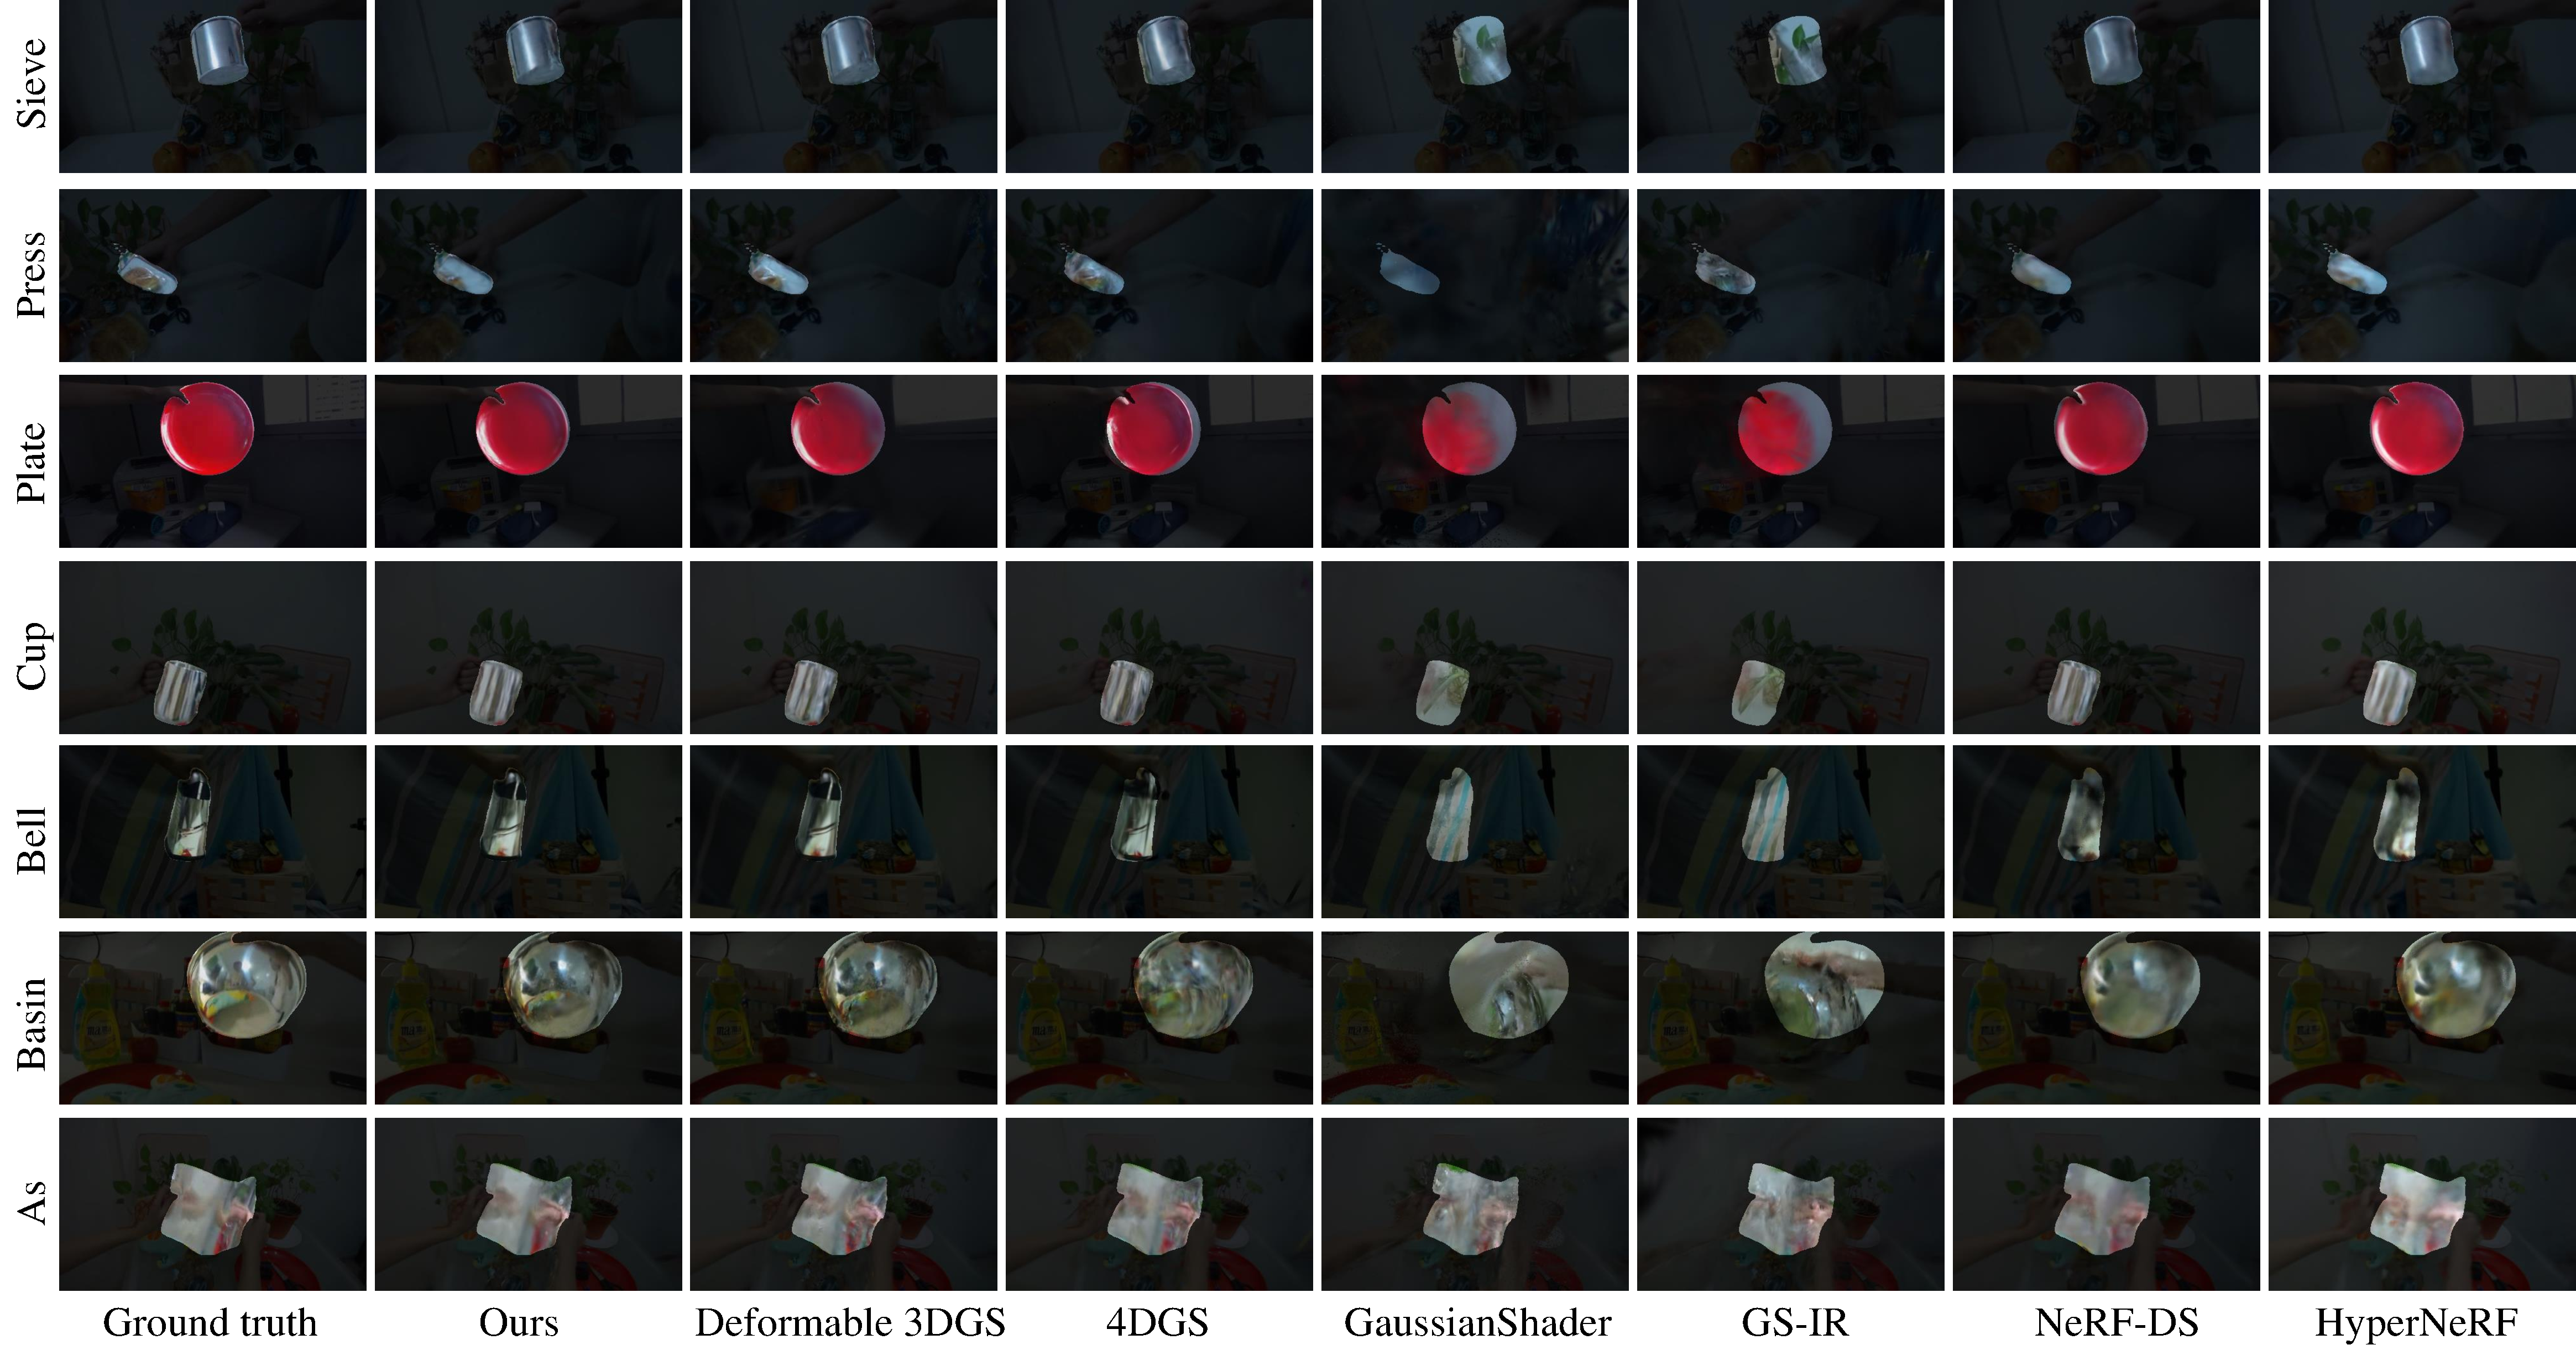
\includegraphics[width=1\linewidth]{figures/mask_appendix_result.pdf}
    \caption{\textbf{Qualitative comparison on NeRF-DS~\citep{yan2023nerf} dataset with labeled dynamic specular masks.}}
    \label{fig:dynamic_spec}
\end{figure*}
Since each scene in the NeRF-DS dataset \citep{yan2023nerf} contains not only dynamic specular objects but also static background objects, we use Track Anything \citep{yang2023track} to obtain masks for the dynamic specular objects. This allows us to evaluate only the dynamic specular objects. As shown in Tab. \ref{tab:dynamic_spec_tab} and Fig. \ref{fig:dynamic_spec}, our method outperforms baselines when evaluating the dynamic specular objects in these monocular sequences.

\subsection{Per-Scene results on the NeRF-DS Dataset}
\begin{figure*}[t]
    \centering
    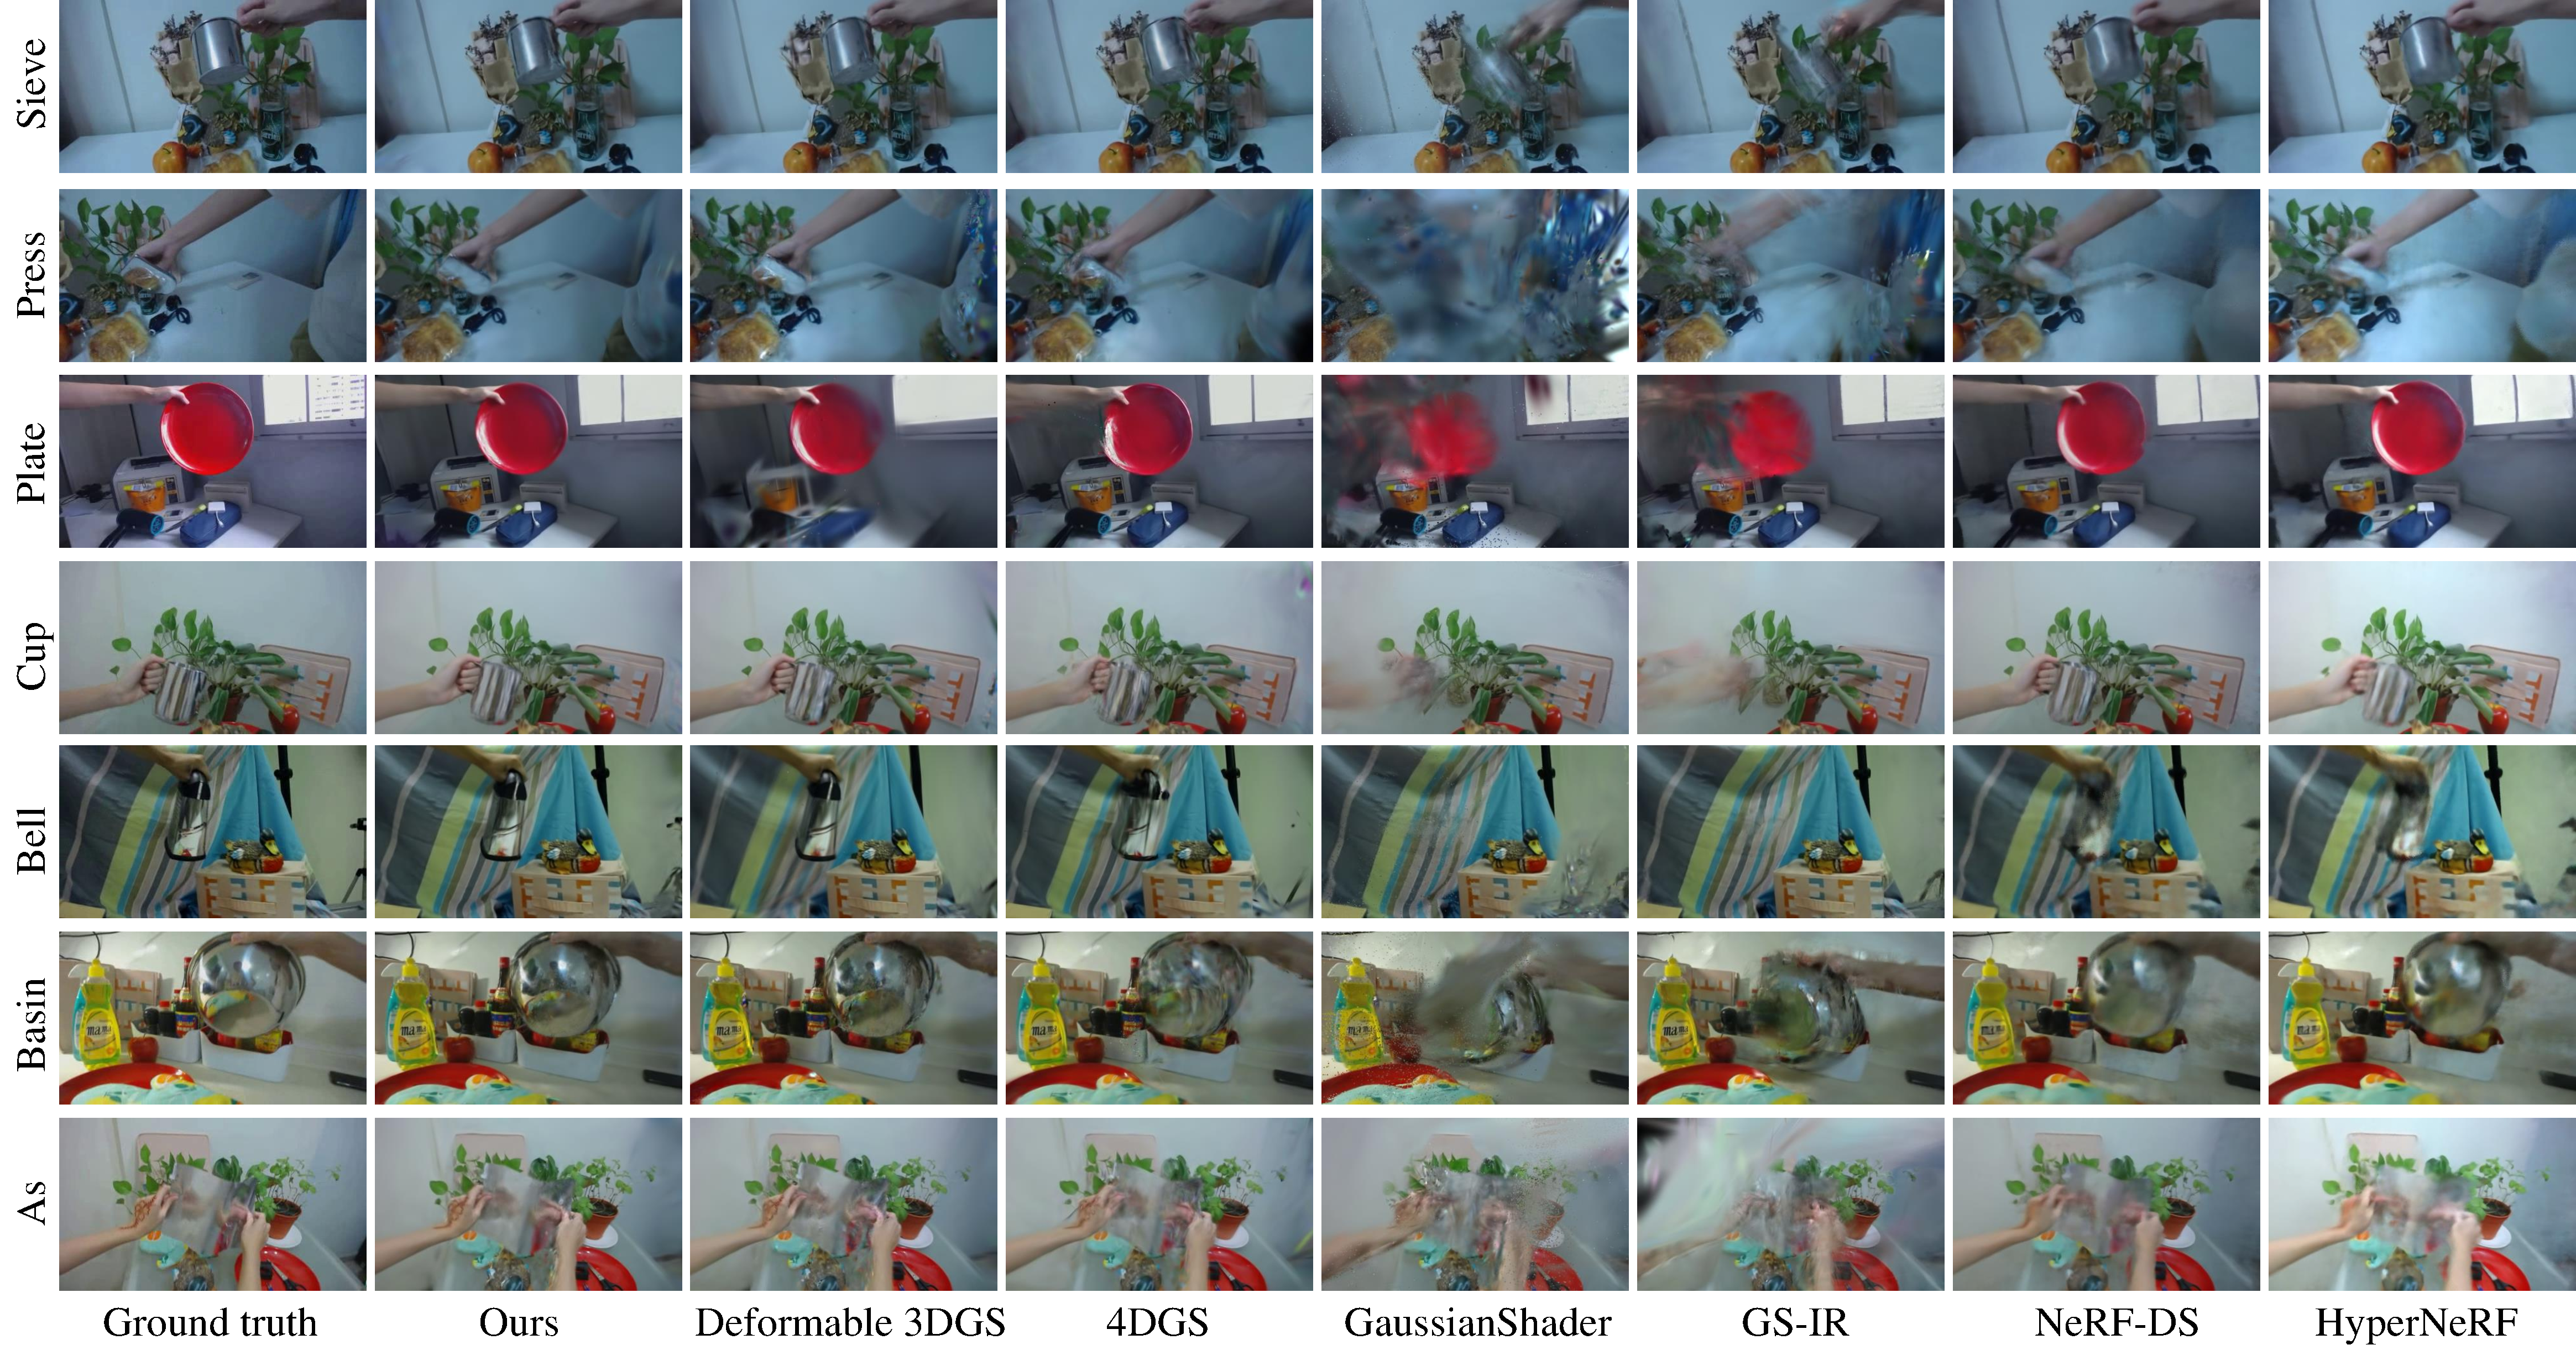
\includegraphics[width=1\linewidth]{figures/rgb_appendix_result.pdf}
    \caption{\textbf{Qualitative comparison on the NeRF-DS~\cite{yan2023nerf} dataset.}}
    \label{fig:whole_scene_appendix}
\end{figure*} 
\begin{figure*}[t]
    \centering
    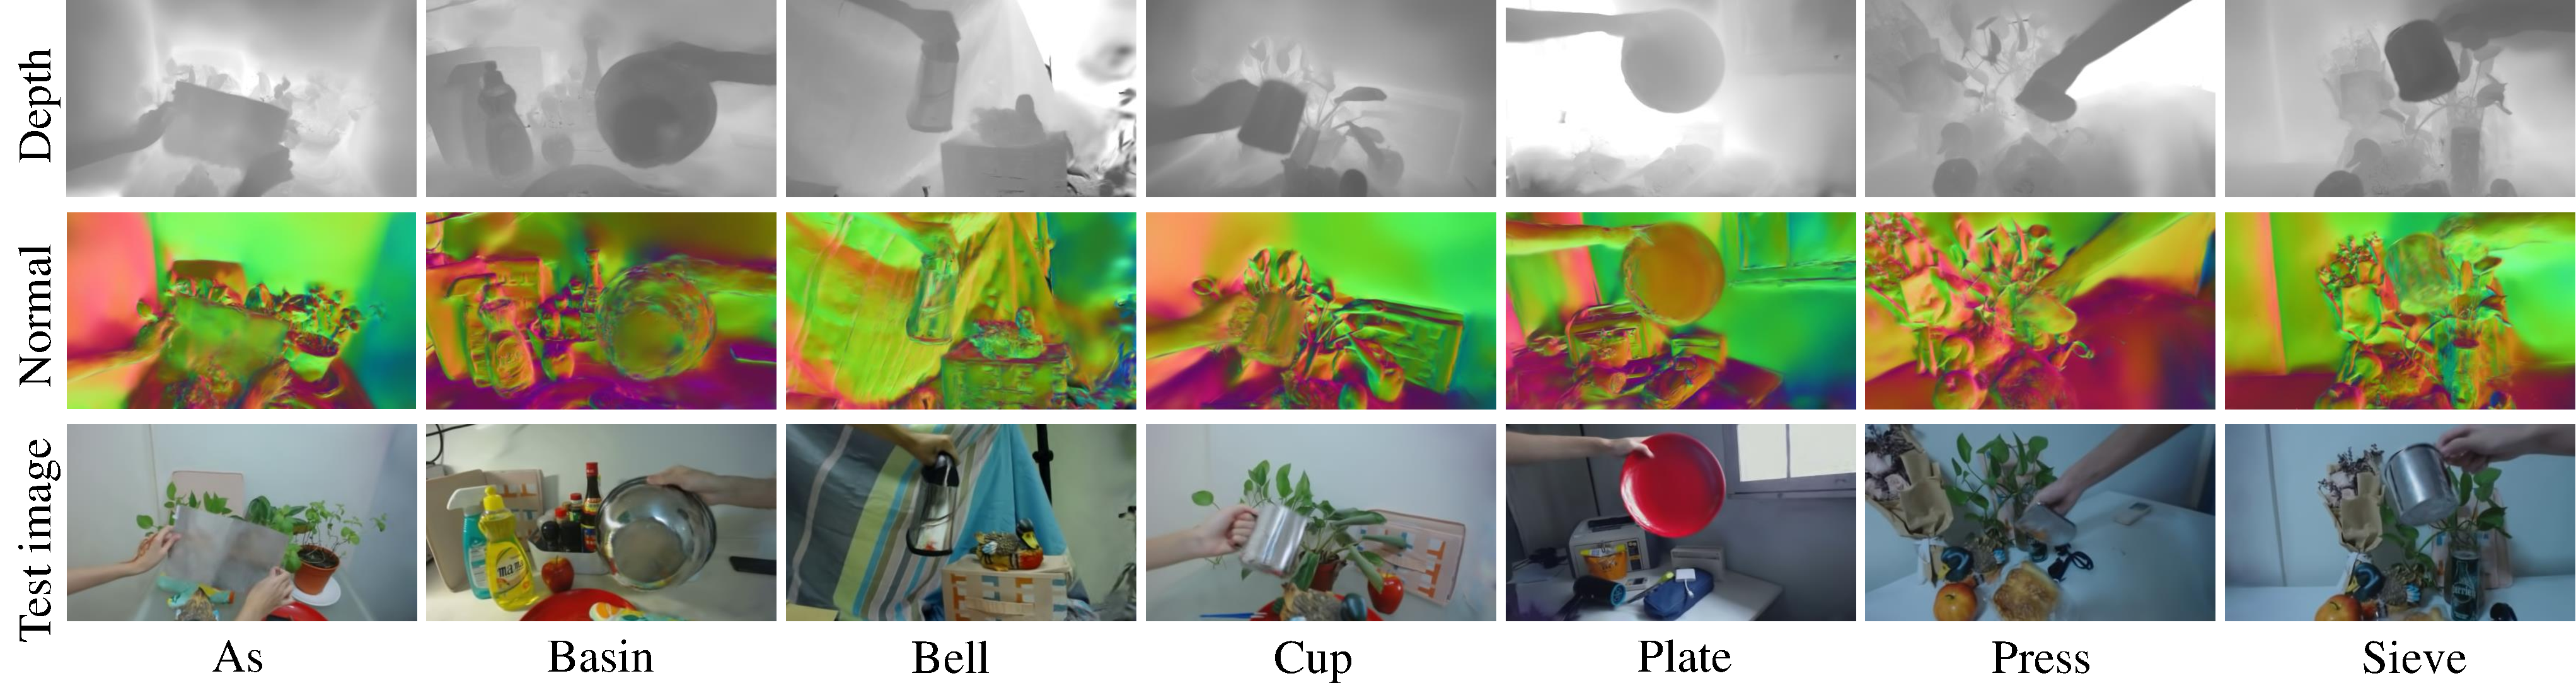
\includegraphics[width=1\linewidth]{figures/rgb_normal_depth.pdf}
    \caption{\textbf{Visualized our rendered test images, normal maps, and depth maps.}}
    \label{fig:rgb_normal_depth}
\end{figure*} 
In Fig. \ref{fig:whole_scene_appendix}, we present qualitative results for each scene in the NeRF-DS dataset \citep{yan2023nerf}. The visualizations demonstrate that our method achieves superior rendering quality compared to other approaches. We also provide rendered test images and their corresponding normal maps and depth maps for each scene in the NeRF-DS dataset in Fig. \ref{fig:rgb_normal_depth}. 


\subsection{Deformation magnitudes and color decomposition}
\begin{figure*}[t]
    \centering    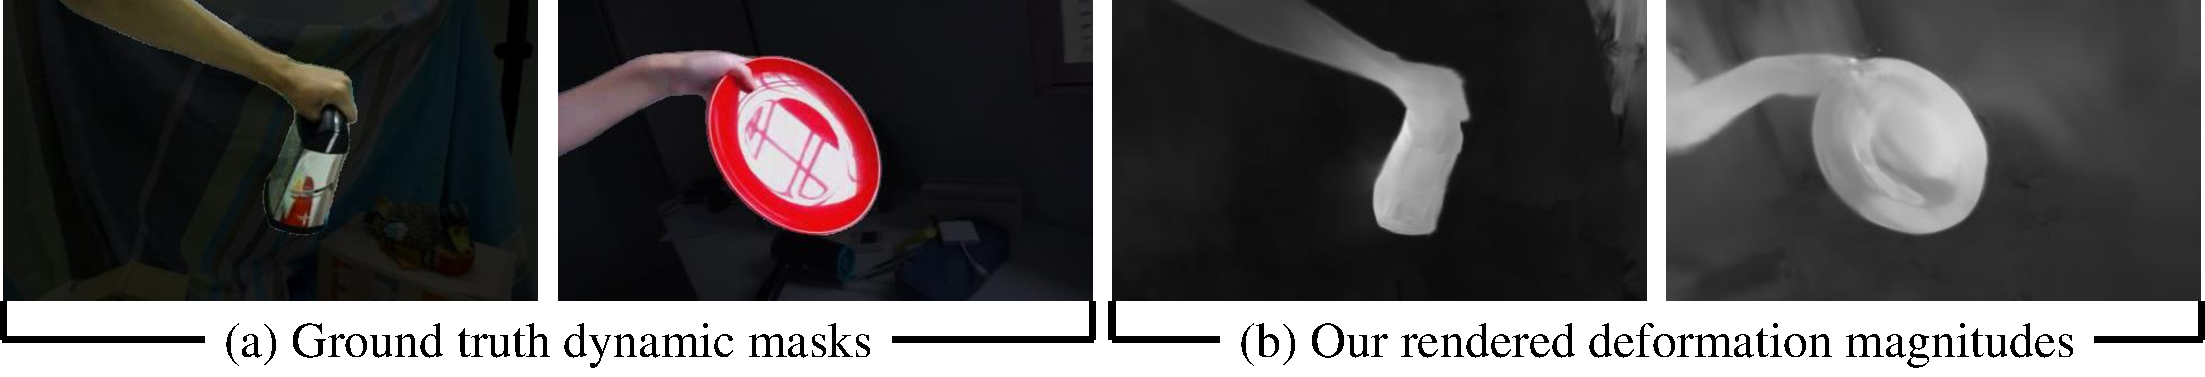
\includegraphics[width=1.0\linewidth]{figures/dynamic_mask.pdf}
    \caption{\textbf{Visualized our deformation magnitudes.} (a) The left side shows the ground truth of the dynamic object, while (b) on the right side, we render the magnitude of the output of the position residual by our deformable Gaussian MLP. The brighter areas indicate greater movement of the 3D Gaussians. The figure shows that even without mask supervision, our method can still effectively distinguish which objects are dynamic.}
    \label{fig:dynamic_mask}
\end{figure*}
\begin{figure*}[t]
    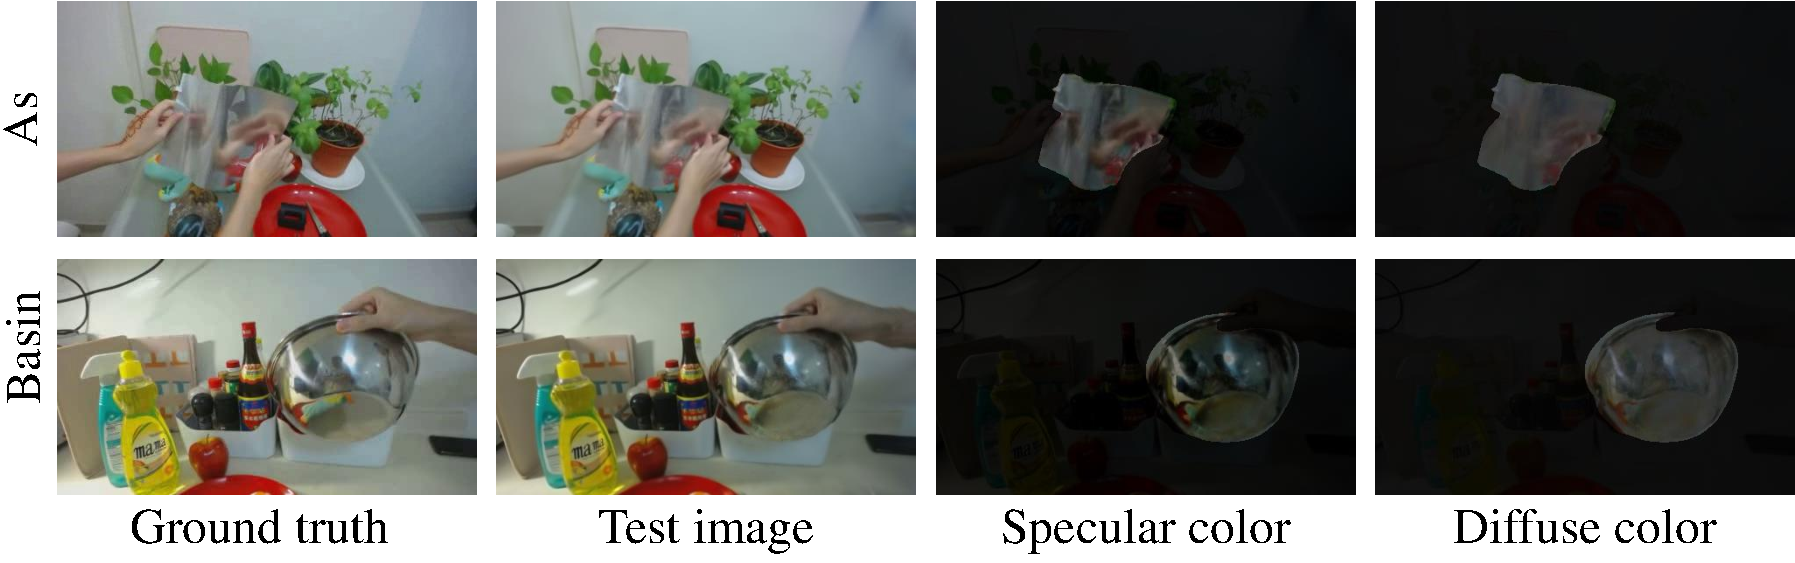
\includegraphics[width=1\linewidth]{figures/decompose.pdf}
    \caption{\textbf{Visualized our specular and diffuse color.} Specular regions are emphasized while non-specular areas are dimmed to highlight the results of specular region color decomposition.}
    \label{fig:decompose}
\end{figure*} 
Unlike NeRF-DS \citep{yan2023nerf}, our approach does not require mask supervision to clearly distinguish between static and dynamic objects, as illustrated in Fig.~\ref{fig:dynamic_mask}. Additionally, Fig.~\ref{fig:decompose} illustrates our method's decomposition results. As shown, our approach consistently achieves a realistic separation of specular and diffuse components across different scenes in the NeRF-DS dataset \citep{yan2023nerf}.

\subsection{Training and rendering efficiency} 
\begin{table}[t]
\centering
\small
\caption{\textbf{Training and rendering efficiency on NeRF-DS~\citep{yan2023nerf} dataset}}
\label{tab:fps}
\begin{tabular}{lccc}
    \toprule
     Scene &  Training time (hr) & FPS & Number of Gaussians (k) \\
    \midrule
    as &1.2  &31  &170  \\
    basin &1.3  &25  &218  \\
    bell &1.9  &18  &335  \\
    cup &1.7  &30 &177  \\
    plate &1.1  &27 &187  \\
    press &1.0  &31 &172  \\
    sieve &1.1  &29 &178  \\
    \bottomrule
\end{tabular}
\end{table}
In Tab. \ref{tab:fps}, we present the training time, FPS, and number of Gaussians from our experiments on each scene in the NeRF-DS dataset \citep{yan2023nerf}. The results show that for scenes with fewer than 178k Gaussians, our method achieves real-time rendering greater than or equal to 30 FPS. The experiments are conducted on an NVIDIA RTX 4090 GPU.


\section{Limitation}~\label{sec:limit}
\begin{figure*}[t]
    \centering
    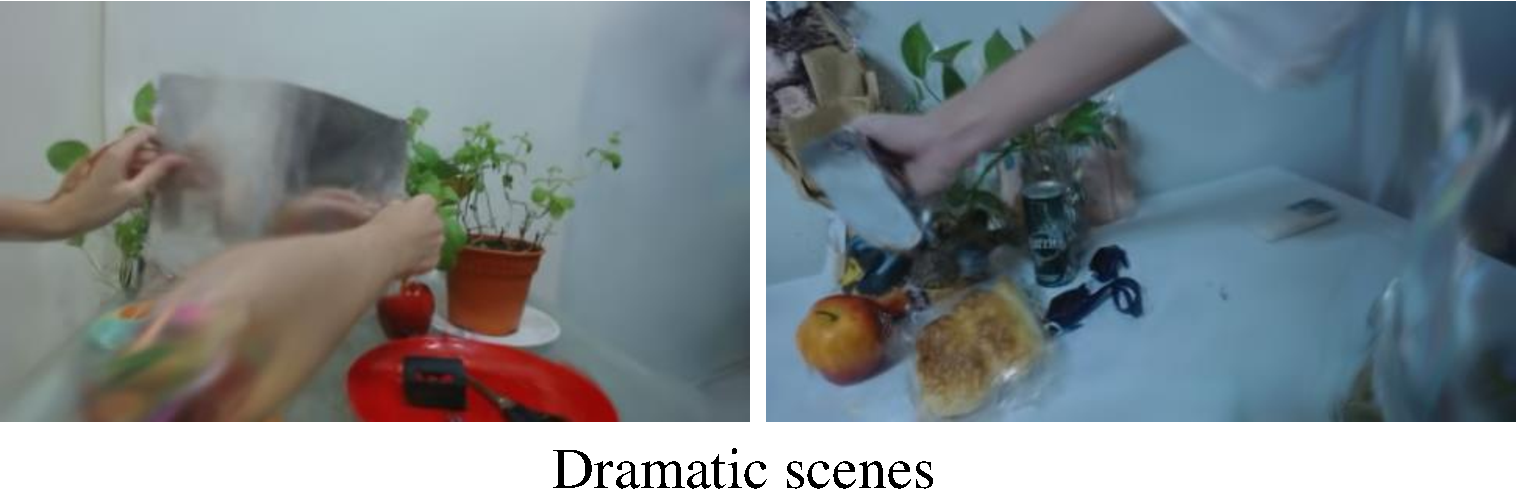
\includegraphics[width=0.8\linewidth]{figures/limit.pdf}
    \caption{\textbf{Failure cases of modeling dramatic scene changes.} There are dramatic scenes where an arm or body enters or exits the scene, leading to many floaters occurring.}
    \label{fig:limit}
\end{figure*}
In some dramatic scenes, relying solely on the deformable Gaussian MLP and coarse-to-fine training strategy is insufficient, such as when an arm or body enters or exits the scene, leading to many floaters occurring. We provide visual results in Fig. \ref{fig:limit}.


